\documentclass[aspectratio=169]{beamer}

% Je kan het lettertype iets vergroten door hierboven optie ``14pt'' toe te
% voegen.

%==============================================================================
% Aanloop
%==============================================================================

%---------- Vormgeving --------------------------------------------------------

\usetheme{hogent}

% Kies hieronder een achtergrondkleur
\usecolortheme{hgwhite} % witte achtergrond, zwarte tekst
%\usecolortheme{hgblack} % zwarte achtergrond, witte tekst

%---------- Packages ----------------------------------------------------------

\usepackage[dutch]{babel}      % Nederlandse taal: splitsingen, enz.

\usepackage{booktabs}          % Mooie tabellen
\usepackage{multirow,multicol} % Tabelcellen samenvoegen
\usepackage{eurosym}           % Euro symbool
\usepackage{qrcode}            % Voor QR-codes op de slotslide
\usepackage{listings}
\usepackage{minted}

%---------- Commando-definities -----------------------------------------------

%---------- Info over de presentatie ------------------------------------------

\title[ITPCO Eindgesprek]{\Large Omzetten van \emph{UML}-diagrammen (\emph{PlantUML}) naar ``\emph{configuration management}''-code (\emph{Ansible}).}
\subtitle{\small Onderzoek \& \emph{Proof of Concept}.}
\author{Lucas Ludueña-Segre}
\date{10 juni, 2026}

%==============================================================================
% Inhoud presentatie
%==============================================================================

\begin{document}

%---------- Titelpagina, inhoudstafel -----------------------------------------

\frame{\maketitle}

\begin{frame}
  \frametitle{Inhoud.}

  \tableofcontents
\end{frame}

%---------- Corpus ------------------------------------------------------------

\section{Introductie.}

\begin{frame}
  \frametitle{\huge Introductie -- Doelgroep.}
  Keuzeprofiel ``\emph{IT infrastructure engineer}''\\(binnen \emph{Toegepaste Informatica})
  \begin{itemize}
    \item Infrastructuren beheren a.d.v.:
          \begin{itemize}
            \item \textbf{Netwerk- en implementatiediagrammen} (\emph{Visual Paradigm} en \emph{draw.io})
            \item \textbf{\emph{Infrastructure-as-Code}} (\emph{Vagrant})
            \item \textbf{\emph{Configuration management}} (\emph{Ansible})
          \end{itemize}
    \item Aangeleerd in de \emph{OLODs}:
          \begin{itemize}
            \item \emph{Cybersecurity Advanced}
            \item \emph{Infrastructure Automation}
            \item \emph{DevOps Project: Operations}
          \end{itemize}
  \end{itemize}
\end{frame}

\begin{frame}
  \frametitle{Introductie -- Probleemstelling.}
  Het proces waarbij \textbf{netwerk- en implementatiediagrammen} geïnterpreteerd en omgezet worden tot ``\emph{IaC}''- en ``\emph{configuration management}''-ondersteunde serveromgevingen is, volgens Nicácio \& Petrillo (2020), \textbf{foutgevoelig} en \textbf{tijdrovend}.
\end{frame}

\begin{frame}
  \frametitle{\huge Introductie -- Hoofdonderzoeksvraag.}
  \textbf{\emph{Hoe kan men een netwerk- en implementatiediagram met minimale menselijke interventie omzetten tot een overeenkomende, gebruiksklare ``}configuration management\emph{''-ondersteunde omgeving?}}
\end{frame}

\begin{frame}
  \frametitle{\Large Introductie -- Deelvragen m.b.t. probleemdomein.}
  \begin{itemize}
    \item Wat zijn de doeleinden (business- of technisch-gericht) van \emph{UML}?
    \item Welke infrastructuur-gerelateerde informatie kan een netwerk- en implementatiediagram \emph{niet} weergeven (dat een \emph{Infrastructure-as-Code}- en/of ``\emph{configuration management}''-tool wel kan)?
    \item Welke stappen zijn er tussen het ontwerp van \emph{UML}-diagrammen en de eerste opstelling van een ``\emph{configuration management}''-ondersteunde omgeving?
  \end{itemize}
\end{frame}

\begin{frame}
  \frametitle{\Large Introductie -- Deelvragen m.b.t. oplossingsdomein.}
  \begin{itemize}
    \item Naast \emph{PlantUML} en \emph{MermaidJS}, met welke andere talen kan men \emph{UML}-diagrammen ontwerpen?
    \item Buiten \emph{Ansible}, \emph{Puppet} en \emph{Chef}, wat zijn andere ``\emph{configuration management}''-tools die voor dit soort doeleinden geschikt zijn?
    \item Aangezien er al tools bestaan om \emph{UML}-diagrammen te genereren op basis van ``\emph{configuration management}''-ondersteunde omgevingen, zoals die van teramako (2023) en rwxd (2025), welke meerwaarde zou deze oplossing (die in de omgekeerde richting werkt) kunnen bieden?
    \item Is het mogelijk om deze oplossing te ontwikkelen a.d.v.\\``\emph{reverse engineering}'' van de bovenstaande tools?
  \end{itemize}
\end{frame}

\section{Methodologie.}

\begin{frame}
  \frametitle{Methodologie -- Fases.}
  \centering
  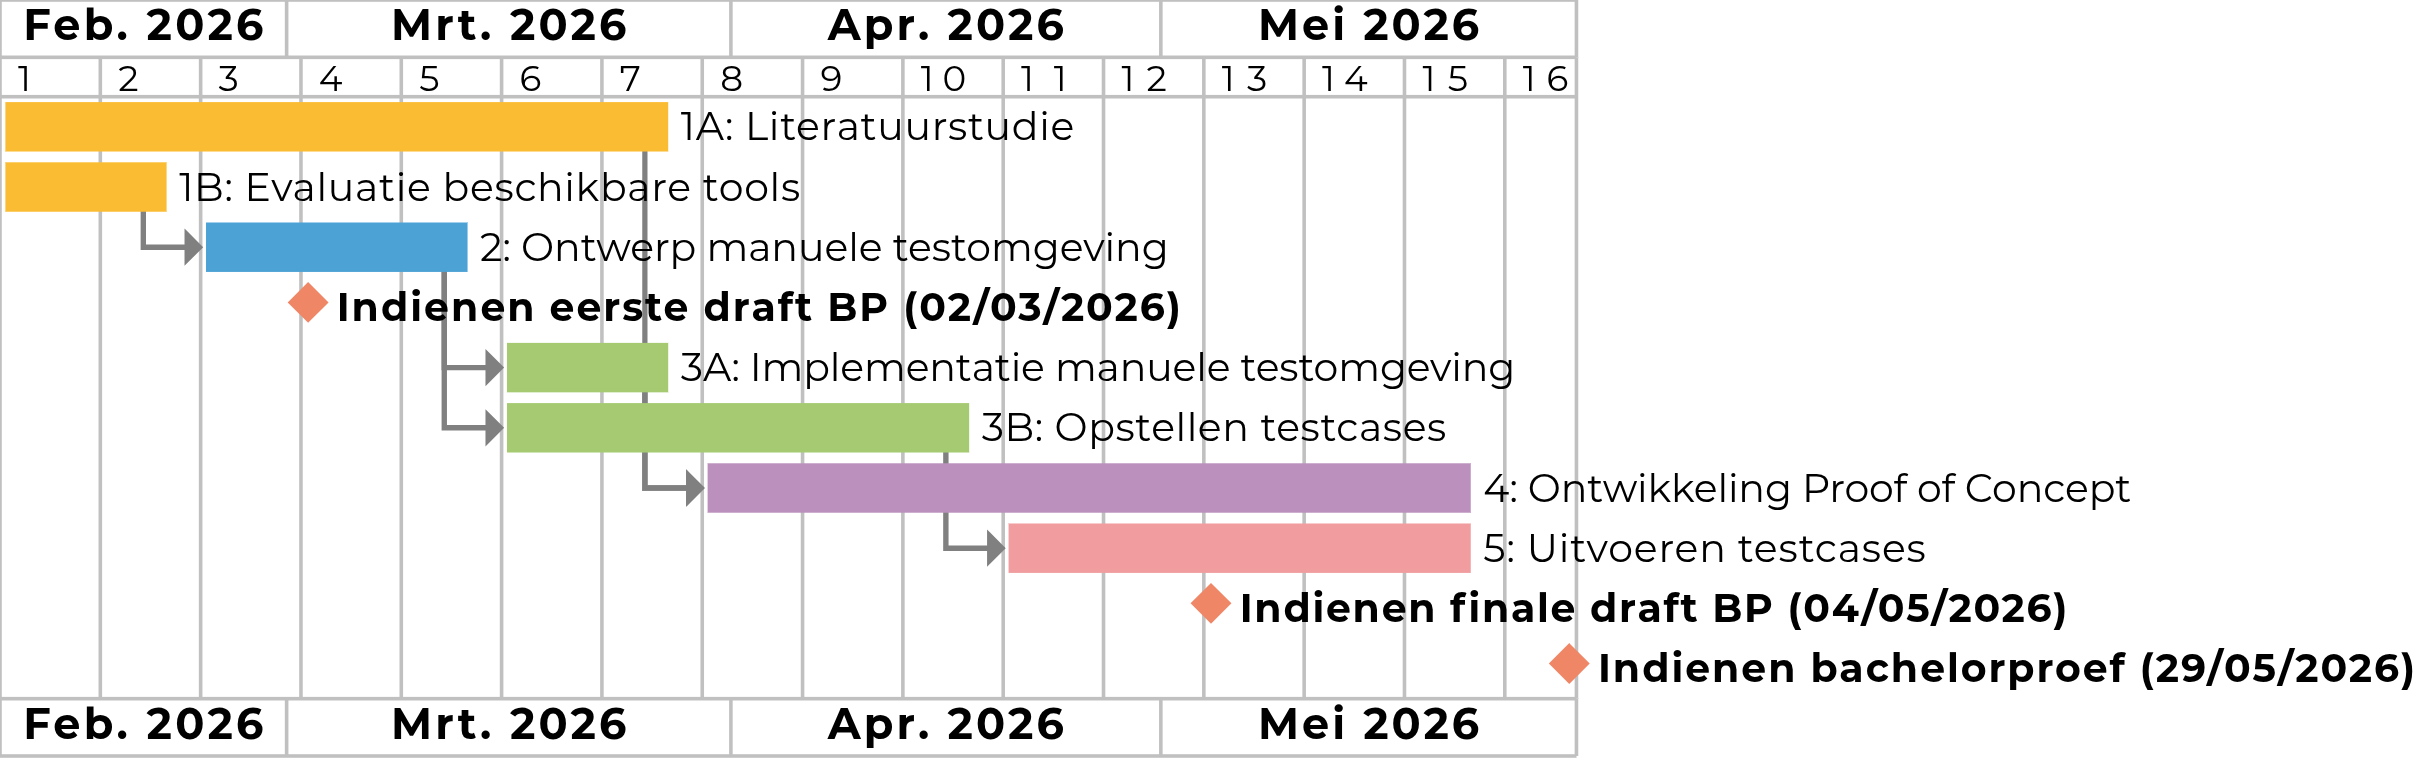
\includegraphics[width=\textwidth]{../graphics/gantt-fases.png}
\end{frame}

\section{Proof of Concept (``\emph{PlantUML2Ansible}'').}

\begin{frame}
  \centering
  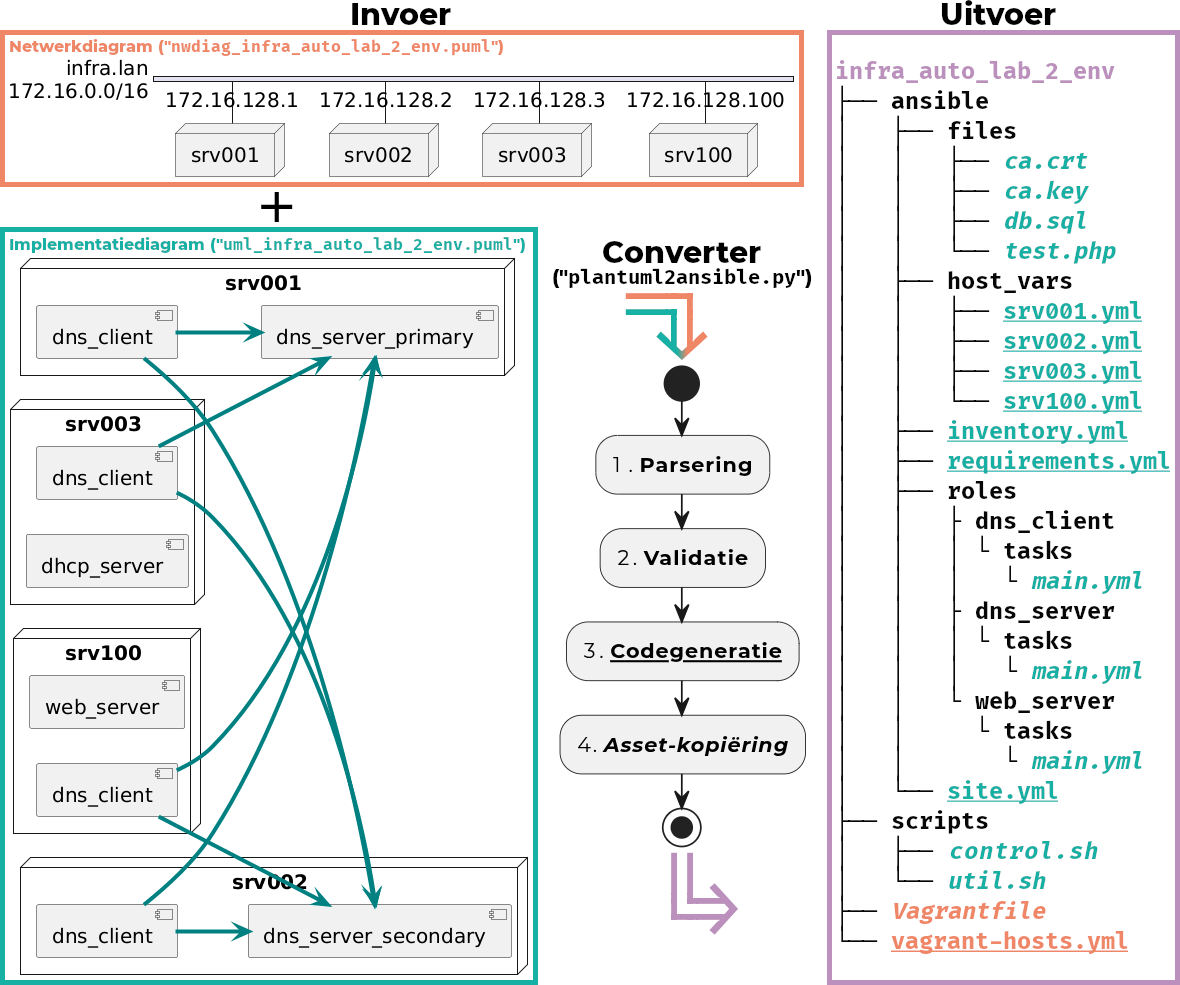
\includegraphics[height=.99\textheight]{../graphics/demo.png}
\end{frame}

\begin{frame}
  \frametitle{\huge Proof of Concept -- Gebruiksscenario's.}
  \centering
  \begin{columns}[t]
    \column{.5\textwidth}
    \textbf{``\textcolor{hgdarkgreen}{\emph{full mode}}''} (``\emph{volledige modus}'')
    \bigskip
    \begin{itemize}
      \item \footnotesize \textbf{Invoer}: netwerk- en implementatiediagram
      \item \footnotesize \textbf{Uitvoer}: \emph{Vagrant}- en \emph{Ansible}-ondersteunde omgeving
      \item Maar \textbf{één netwerk} mogelijk
    \end{itemize}

    \column{.5\textwidth}
    \small \textbf{``\textcolor{hgorange}{\emph{IaC-only-mode}}''} (``\emph{enkel-IaC-modus}'')
    \bigskip
    \begin{itemize}
      \item \footnotesize \textbf{Invoer}: netwerkdiagram
      \item \footnotesize \textbf{Uitvoer}: \emph{Vagrant}-ondersteunde omgeving
      \item \textbf{Meerdere netwerken} mogelijk\\(max. 3 IP-adressen per host)
    \end{itemize}
  \end{columns}
\end{frame}

\section{Resultaten.}
\begin{frame}
  \frametitle{\normalsize Resultaten -- Testcase 1 -- \emph{Cybersecurity Advanced} (``\textbf{\textcolor{hgorange}{\emph{IaC-only-mode}}}'').}
  \centering
  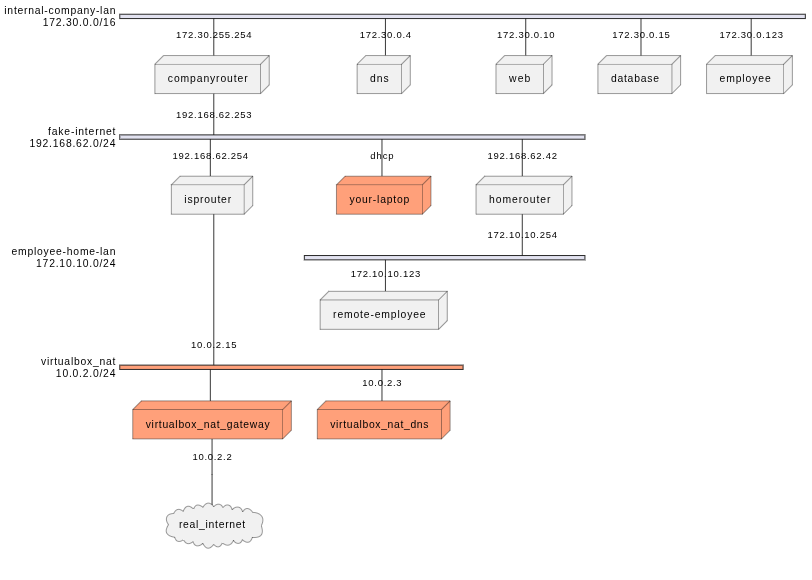
\includegraphics[width=.7\textwidth]{../graphics/nwdiag_cybersec_adv_env.png}
\end{frame}

\begin{frame}
  \frametitle{\normalsize Resultaten -- Testcase 1 -- \emph{Cybersecurity Advanced} (``\textbf{\textcolor{hgorange}{\emph{IaC-only-mode}}}'').}
  \begin{columns}[t]
    \column{.5\textwidth}
    \textbf{Gegenereerde bestanden:}
    \begin{itemize}
      \item \footnotesize ``\texttt{vagrant-hosts.yml}''
    \end{itemize}
    \column{.5\textwidth}
    \textbf{Gekopieerde assets:}
    \begin{itemize}
      \item \footnotesize ``\texttt{Vagrantfile}''
    \end{itemize}
  \end{columns}
\end{frame}

\begin{frame}
  \frametitle{\normalsize Resultaten -- Testcase 1 -- \emph{Cybersecurity Advanced} (``\textbf{\textcolor{hgorange}{\emph{IaC-only-mode}}}'').}
  \begin{columns}[t]
    \column{.6\textwidth}
    ``\texttt{nwdiag\_cybersec\_adv\_env.puml}'' \texttt{==>}
    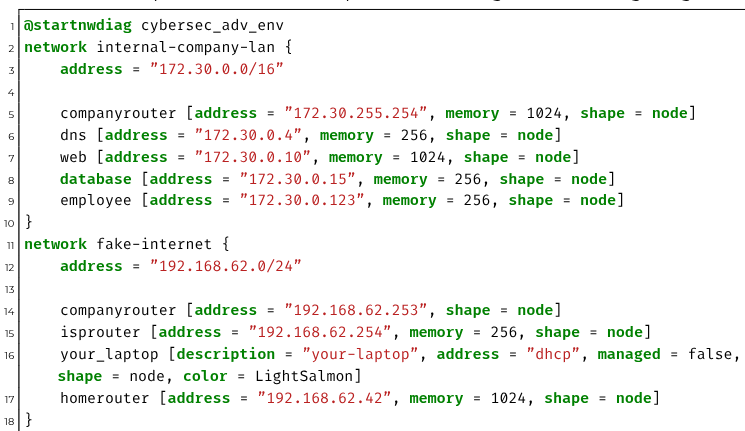
\includegraphics[width=\textwidth]{../graphics/presentatie_vb_1.png}

    \column{.4\textwidth}
    ``\texttt{vagrant-hosts.yml}''
    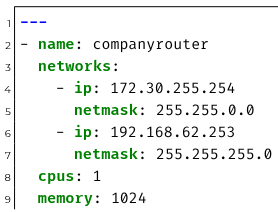
\includegraphics[width=.6\textwidth]{../graphics/presentatie_vb_2.png}
  \end{columns}
\end{frame}


\begin{frame}
  \frametitle{\normalsize Resultaten -- Testcase 2 -- \emph{Infrastructure Automation}, labo 2 (``\textbf{\textcolor{hgdarkgreen}{\emph{full mode}}}'').}
  \centering
  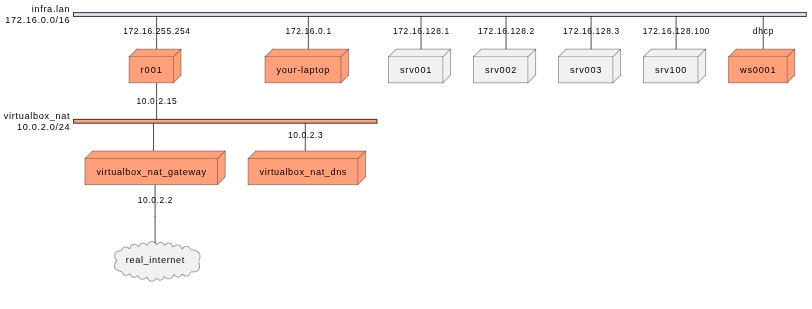
\includegraphics[width=\textwidth]{../graphics/nwdiag_infra_auto_lab_2_env.png}
\end{frame}

\begin{frame}
  \frametitle{\normalsize Resultaten -- Testcase 2 -- \emph{Infrastructure Automation}, labo 2 (``\textbf{\textcolor{hgdarkgreen}{\emph{full mode}}}'').}
  \centering
  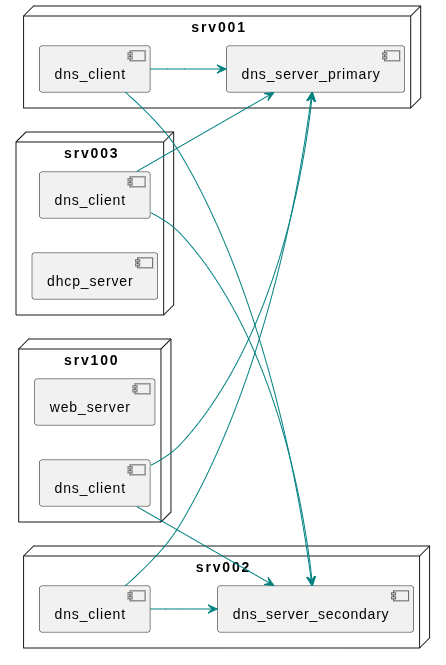
\includegraphics[height=.8\textheight]{../graphics/uml_infra_auto_lab_2_env.png}
\end{frame}

\begin{frame}
  \frametitle{\normalsize Resultaten -- Testcase 2 -- \emph{Infrastructure Automation}, labo 2 (``\textbf{\textcolor{hgdarkgreen}{\emph{full mode}}}'').}
  \begin{columns}[t]
    \column{.5\textwidth}
    \textbf{Gegenereerde bestanden:}
    \begin{itemize}
      \item \footnotesize ``\texttt{vagrant-hosts.yml}''
      \item \footnotesize ``\texttt{ansible/inventory.yml}''
      \item \footnotesize ``\texttt{ansible/site.yml}''
      \item \footnotesize ``\texttt{ansible/host\_vars/\ldots}''
            \begin{itemize}
              \item \footnotesize ``\texttt{\ldots srv001.yml}''
              \item \footnotesize ``\texttt{\ldots srv002.yml}''
              \item \footnotesize ``\texttt{\ldots srv003.yml}''
              \item \footnotesize ``\texttt{\ldots srv100.yml}''
            \end{itemize}
      \item \footnotesize ``\texttt{ansible/requirements.yml}''
    \end{itemize}
    \bigskip
    \column{.5\textwidth}
    \textbf{Gekopieerde assets:}
    \begin{itemize}
      \item \footnotesize ``\texttt{Vagrantfile}''
      \item \footnotesize ``\texttt{scripts/}''
      \item \footnotesize ``\texttt{ansible/roles/\ldots}''
            \begin{itemize}
              \item \footnotesize ``\texttt{\ldots web\_server/}''
              \item \footnotesize ``\texttt{\ldots dns\_server/}''
              \item \footnotesize ``\texttt{\ldots dns\_client/}''
            \end{itemize}
      \item \footnotesize ``\texttt{ansible/files/\ldots}''
            \begin{itemize}
              \item \footnotesize ``\texttt{\ldots ca.crt}''*
              \item \footnotesize ``\texttt{\ldots ca.key}''*
              \item \footnotesize ``\texttt{\ldots db.sql}''
              \item \footnotesize ``\texttt{\ldots test.php}''
            \end{itemize}
    \end{itemize}
    \scriptsize (*): optionele bestanden voor HTTPS-ondersteuning
  \end{columns}
\end{frame}

\begin{frame}
  \frametitle{\large Resultaten -- Testcase 2: uitvoer (voorbeeld)}
  \begin{columns}[t]
    \column{.6\textwidth}
    ``\texttt{uml\_infra\_auto\_lab\_2\_env.puml}'' \texttt{==>}

    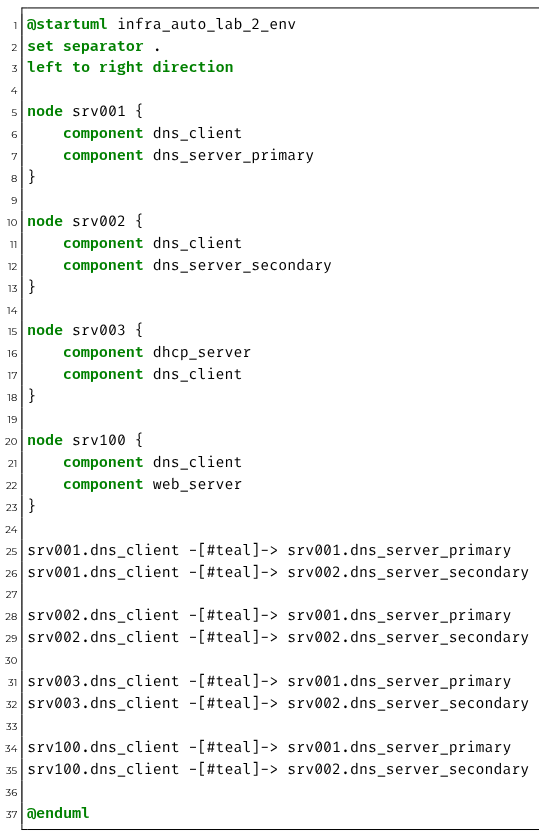
\includegraphics[height=.7\textheight]{../graphics/presentatie_vb_3.png}

    \column{.4\textwidth}
    ``\texttt{site.yml}''

    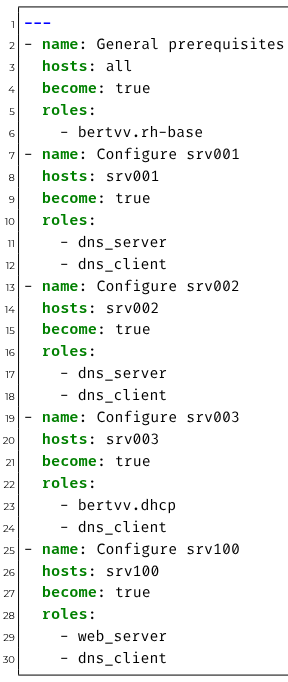
\includegraphics[height=.7\textheight]{../graphics/presentatie_vb_4.png}
  \end{columns}
\end{frame}

\begin{frame}
  \frametitle{\normalsize Resultaten -- Testcase 3 -- \emph{Infrastructure Automation}, labo 3 (``\textbf{\textcolor{hgdarkgreen}{\emph{full mode}}}'').}
  \centering
  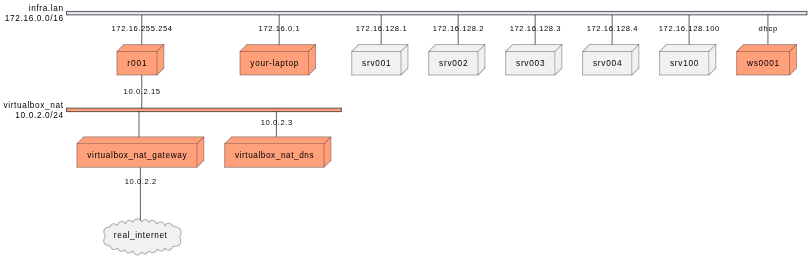
\includegraphics[width=\textwidth]{../graphics/nwdiag_infra_auto_lab_3_env.png}
\end{frame}

\begin{frame}
  \frametitle{\normalsize Resultaten -- Testcase 3 -- \emph{Infrastructure Automation}, labo 3 (``\textbf{\textcolor{hgdarkgreen}{\emph{full mode}}}'').}
  \centering
  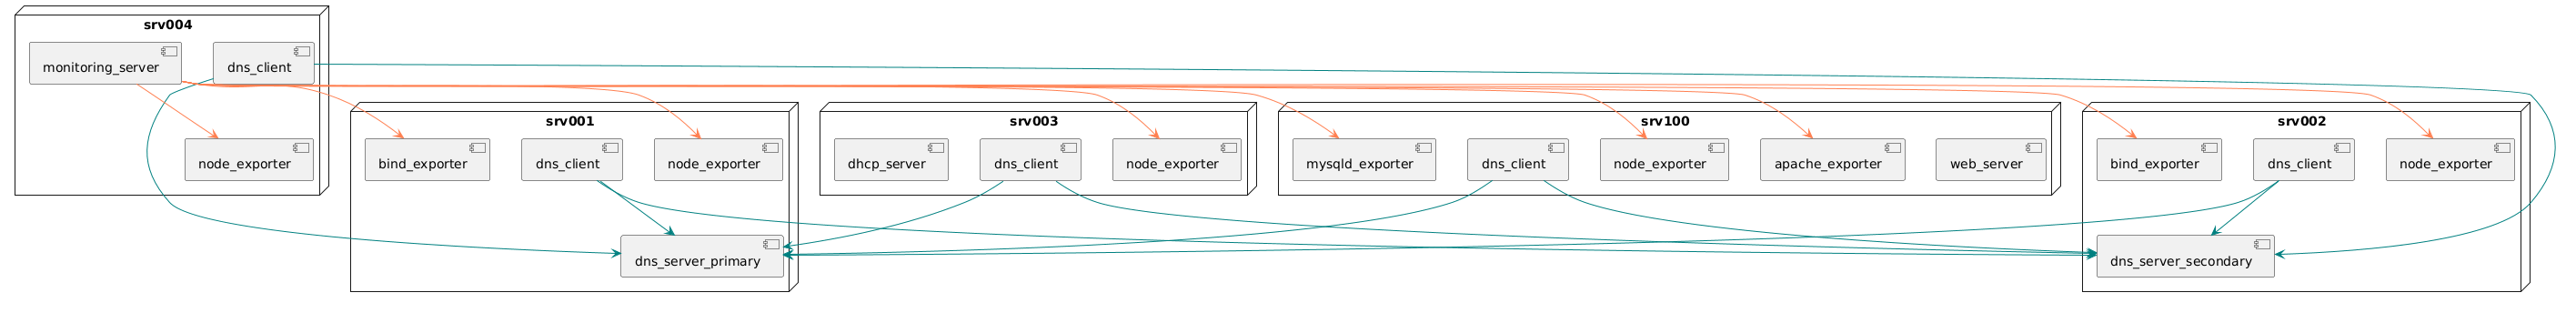
\includegraphics[width=\textwidth]{../graphics/uml_infra_auto_lab_3_env_horizontal.png}
\end{frame}

\begin{frame}
  \frametitle{\normalsize Resultaten -- Testcase 3 -- \emph{Infrastructure Automation}, labo 3 (``\textbf{\textcolor{hgdarkgreen}{\emph{full mode}}}'').}
  \begin{columns}[t]
    \column{.5\textwidth}
    \textbf{Gegenereerde bestanden:}
    \begin{itemize}
      \item \footnotesize ``\texttt{ansible/host\_vars/srv004.yml}''
      \item \footnotesize ``\texttt{ansible/requirements.yml}'' \\\scriptsize (+ ``\texttt{prometheus.prometheus}''- en ``\texttt{grafana.grafana}''-``\emph{Ansible Galaxy}''-collecties)
      \item \footnotesize ``\texttt{ansible/host\_vars/\ldots}''
            \begin{itemize}
              \item \footnotesize ``\texttt{\ldots srv001.yml}''
              \item \footnotesize ``\texttt{\ldots srv002.yml}''
              \item \footnotesize ``\texttt{\ldots srv100.yml}''
            \end{itemize}
            \scriptsize (uitgebreid voor ````\texttt{bind\_exporter}'', \texttt{apache\_exporter}'' \& ``\texttt{mysqld\_exporter}'')
      \item \footnotesize \ldots (overige gegenereerde bestanden van testcase 2)
    \end{itemize}
    \column{.6\textwidth}
    \textbf{Gekopieerde assets:}
    \begin{itemize}
      \item \footnotesize ``\texttt{ansible/roles/monitoring\_server/}''
      \item \footnotesize ``\texttt{ansible/files/grafana/default.yml}''
      \item \footnotesize ``\texttt{ansible/files/grafana/dashboards/\ldots}''
            \begin{itemize}
              \item \footnotesize ``\texttt{\ldots apache\_exporter.json}''
              \item \footnotesize ``\texttt{\ldots bind\_exporter.json}''
              \item \footnotesize ``\texttt{\ldots mysqld\_exporter.json}''
              \item \footnotesize ``\texttt{\ldots node\_exporter.json}''
            \end{itemize}
      \item \footnotesize \ldots (overige gekopieerde assets van testcase 2)
    \end{itemize}
  \end{columns}
\end{frame}

\begin{frame}
  \frametitle{\normalsize Resultaten -- Testcase 3 -- \emph{Infrastructure Automation}, labo 3 (``\textbf{\textcolor{hgdarkgreen}{\emph{full mode}}}'').}
  \footnotesize ``\texttt{uml\_infra\_auto\_lab\_3\_env.puml}'' \texttt{==>} ``\texttt{ansible/host\_vars/srv004.yml}''
  \begin{columns}[t]
    \column{.6\textwidth}

    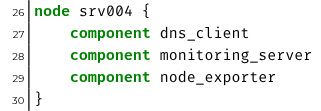
\includegraphics[height=.2\textheight]{../graphics/presentatie_vb_5.png}

    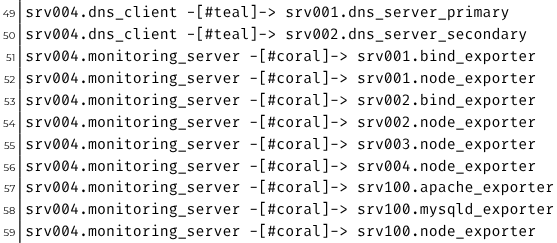
\includegraphics[height=.45\textheight]{../graphics/presentatie_vb_6.png}

    \column{.4\textwidth}
    \medskip

    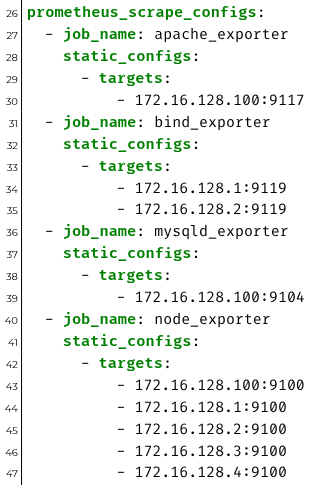
\includegraphics[height=.65\textheight]{../graphics/presentatie_vb_7.png}
  \end{columns}
\end{frame}

\section{Conclusie.}

\begin{frame}
  \frametitle{Conclusie.}
  \begin{itemize}
    \item Het is \textbf{technisch haalbaar} om op basis van netwerk- en implementatiediagrammen functionele omgevingen te produceren \textbf{zonder manuele tussenkomst}.
    \item De \textbf{kloof tussen de ontwerp- en implementatiefase} wordt met deze tool aanzienlijk \textbf{verkleind}, alsook de kans op \textbf{menselijke fouten}.
    \item De meerwaarde van deze tool bevindt zich binnen een \textbf{educatieve context}, zowel voor docenten als studenten.
  \end{itemize}
  \centering
\end{frame}

\begin{frame}
  \frametitle{\LARGE Conclusie -- Beperkingen en uitbreidingen.}
  \centering
  \begin{columns}[t]
    \column{.5\textwidth}
    \textbf{Beperkingen van de \emph{converter}}:
    \begin{itemize}
      \item[\textcolor{hgorange}{\large \textbf{-- }}] \footnotesize Eén netwerk binnen ``\textcolor{hgdarkgreen}{\textbf{\emph{full mode}}}''.
      \item[\textcolor{hgorange}{\large \textbf{-- }}] \footnotesize Geen routering tussen verschillende netwerken.
      \item[\textcolor{hgorange}{\large \textbf{-- }}] \footnotesize Enkel \emph{IPv4}-adressering.
      \item[\textcolor{hgorange}{\large \textbf{-- }}] \footnotesize Alleen \emph{AlmaLinux 9} als gastbesturingssysteem.
      \item[\textcolor{hgorange}{\large \textbf{-- }}] \footnotesize Beperkte subset van de \emph{PlantUML}-syntax ondersteund.
    \end{itemize}

    \column{.55\textwidth}
    \textbf{Mogelijke toekomstige uitbreidingen}:
    \begin{itemize}
      \item[\textcolor{hglightgreen}{\large \textbf{+ }}] \footnotesize Meerdere netwerken binnen ``\textcolor{hgdarkgreen}{\textbf{\emph{full mode}}}'' \\(+ routering \& firewall-regels).
      \item[\textcolor{hglightgreen}{\large \textbf{+ }}] \footnotesize \emph{IPv6}-adressering.
      \item[\textcolor{hglightgreen}{\large \textbf{+ }}] \footnotesize Uitbreiding naar andere gastbesturingssystemen.
      \item[\textcolor{hglightgreen}{\large \textbf{+ }}] \footnotesize Geïntegreerde linters voor validatie \\van invoer en uitvoer.
      \item[\textcolor{hglightgreen}{\large \textbf{+ }}] \footnotesize Andere \emph{IaC-} en \emph{configuration management}-\emph{backends}.
    \end{itemize}
  \end{columns}
\end{frame}

\begin{frame}
  \frametitle{Broncode.}
  \begin{columns}[c]
    \column{.5\textwidth}
    \centering
    \textbf{Broncode bachelorproef (\emph{LaTeX})}
    \bigskip\\
    \qrcode[height=3cm]{https://github.com/lucasluduenasegre/latex-hgbachproef-nl-25-26-luduenasegrelucas}\\

    \column{.5\textwidth}
    \centering
    \textbf{Broncode ``\emph{PlantUML2Ansible}''}
    \bigskip\\
    \qrcode[height=3cm]{https://github.com/lucasluduenasegre/plantuml2ansible}\\
  \end{columns}
\end{frame}

\begin{frame}
  \centering
  \Huge \textbf{Bedankt! Vragen?}
\end{frame}

\end{document}
